\documentclass[11pt, a4paper]{article}
\usepackage[utf8]{inputenc}
\usepackage[left=2.35cm, right=3.35cm, top=3.35cm, bottom=3.0cm]{geometry}
\usepackage{amsmath, amssymb, amsthm}
\usepackage[english]{babel}
\usepackage{graphicx}
\usepackage[font={small,it}]{caption}
\graphicspath{ {figures/} }
\usepackage{url}
\usepackage{appendix}
\usepackage{float}
\usepackage[bottom]{footmisc}
\usepackage{titling}
\setlength{\droptitle}{-10em}  

\title{ \huge Artificial neural networks \\ 
  { \large Assignment 1: Supervised learning and generalization }}
\author{
        Lood, Cedric
}

\begin{document}
\maketitle
%\tableofcontents

\section{Context}

Artificial neural networks that have at least 1 hidden layer have the
property of being universal
approximator\cite{hornik1989multilayer,leshno1993multilayer}. Hence,
any non-linear function can be realized using classical feedforward
multilayers networks. In this assignment, we were asked to explore the
different training algorithms that can be used with backpropagation in
order to learn non-linear functions. These function have different
yields in terms of performance, training time, and more importantly
generalization. Some comparisons of the approaches are explored in
this report.

\noindent For illustration purposes, I worked with 2 functions
illustrated here (graphics created using ggplot2 and R \footnote{All
  matlab and R code can be found online at:
  https://github.com/milt0n/ANN-Experiments}):

\begin{itemize}
\item A simple polynomial function with equation $f(x)=x^3-11x+2$
  illustrated on the left of figure \ref{fig:functions}.
\item A more \emph{``wiggle-y''} function, that exhibits some
  dampening, with equation $g(x)=e(-x^2)sin(10x)$ illustrated on the
  the right of figure \ref{fig:functions}.
\end{itemize}

\begin{figure}[H]
    \centering
    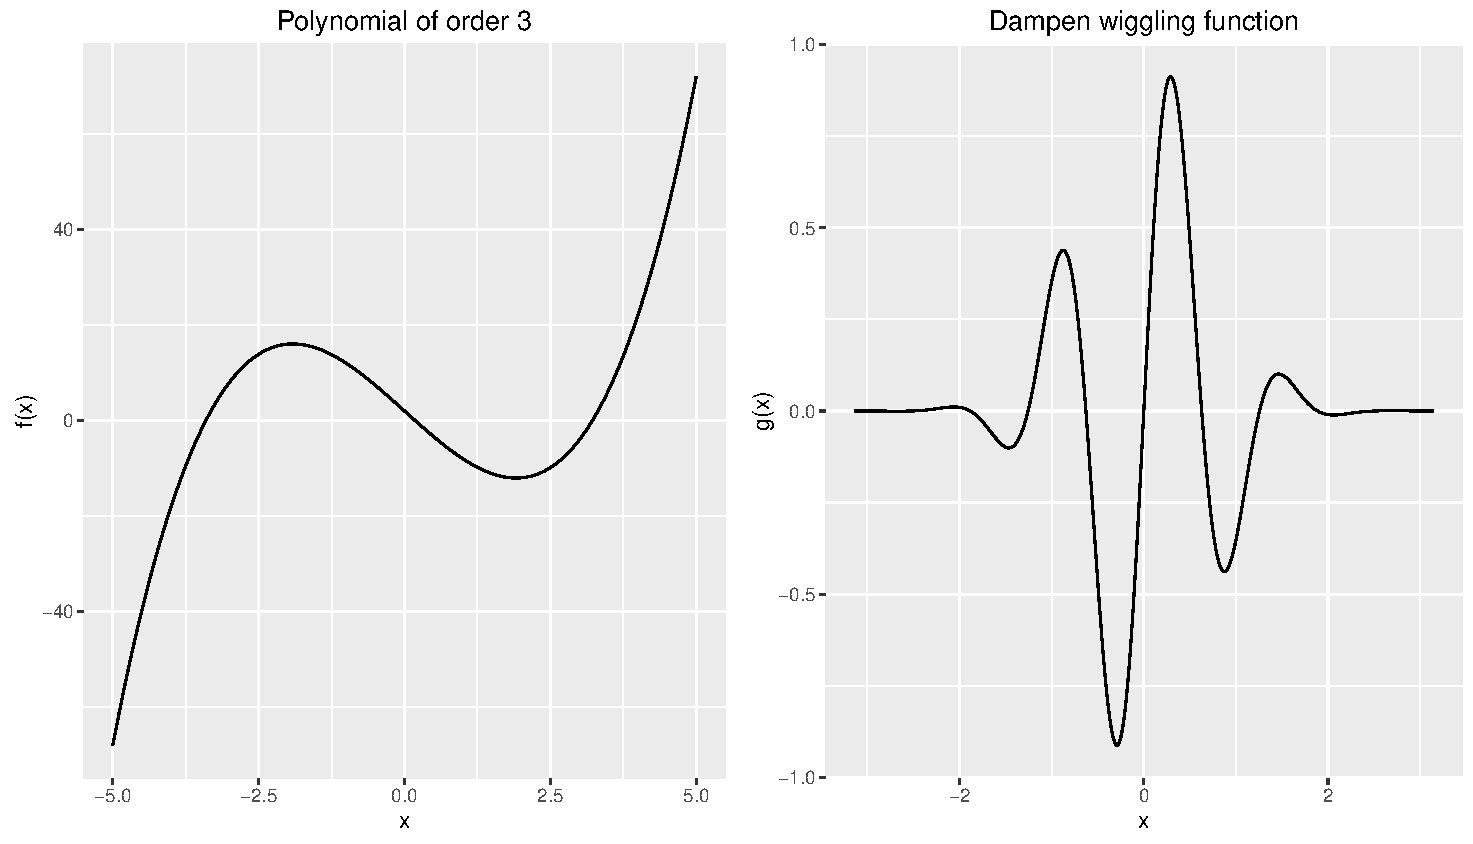
\includegraphics[scale=.65]{true_functions.pdf}
    \caption{Graphs of the underlying true functions used in the analysis}
    \label{fig:functions}
\end{figure}

\section{Noise-free learning}
In this section, we explore the learning in a supervised manner of a
dataset produced by a known underlying function. The entry for the
learning algorithm is thus a set of tuples $(x, y)$ with $x$ chosen
over a given interval, and $y=f(x)$.

The architecture chosen for the feedforward multilayer neural net
consisted of 1 hidden layer, with 10 neurons, and 1 neuron in the
output layer. The transfer function for the hidden layer neurons is
the sigmoid, and the output neuron has a linear transfer function
$f(x)=x$. 

On figure \ref{fig:traingd}, one can see that the training of the
neural net using gradient descent (\emph{traingd} in matlab) had very
poor result. 

\begin{description}
\item [top graph] that represents the polynomial function
  $f(x)=x^3-11x+2$ performed the worst, with a problem of computation
  of the gradient during the training. The gradient at each
  \emph{epoch} of the training becomes larger and larger, and
  eventually too large to represent (\emph{NaN} in matlab), and the
  training fails so I kept it below 50 \emph{epochs}.
\item [bottom graph] the gradient descent performed a little bit
  better on $g(x)=e(-x^2)sin(10x)$ but the performance were still not
  satisfying in terms of approximation. I tried raising the number of
  \emph{epochs} to 10000 and 100000 but the behaviour there was that
  the approximation was getting closer and closer to a flat function
  like $y = 0$, hence traversing 
\end{description}

\begin{figure}[H]
  % \centering
  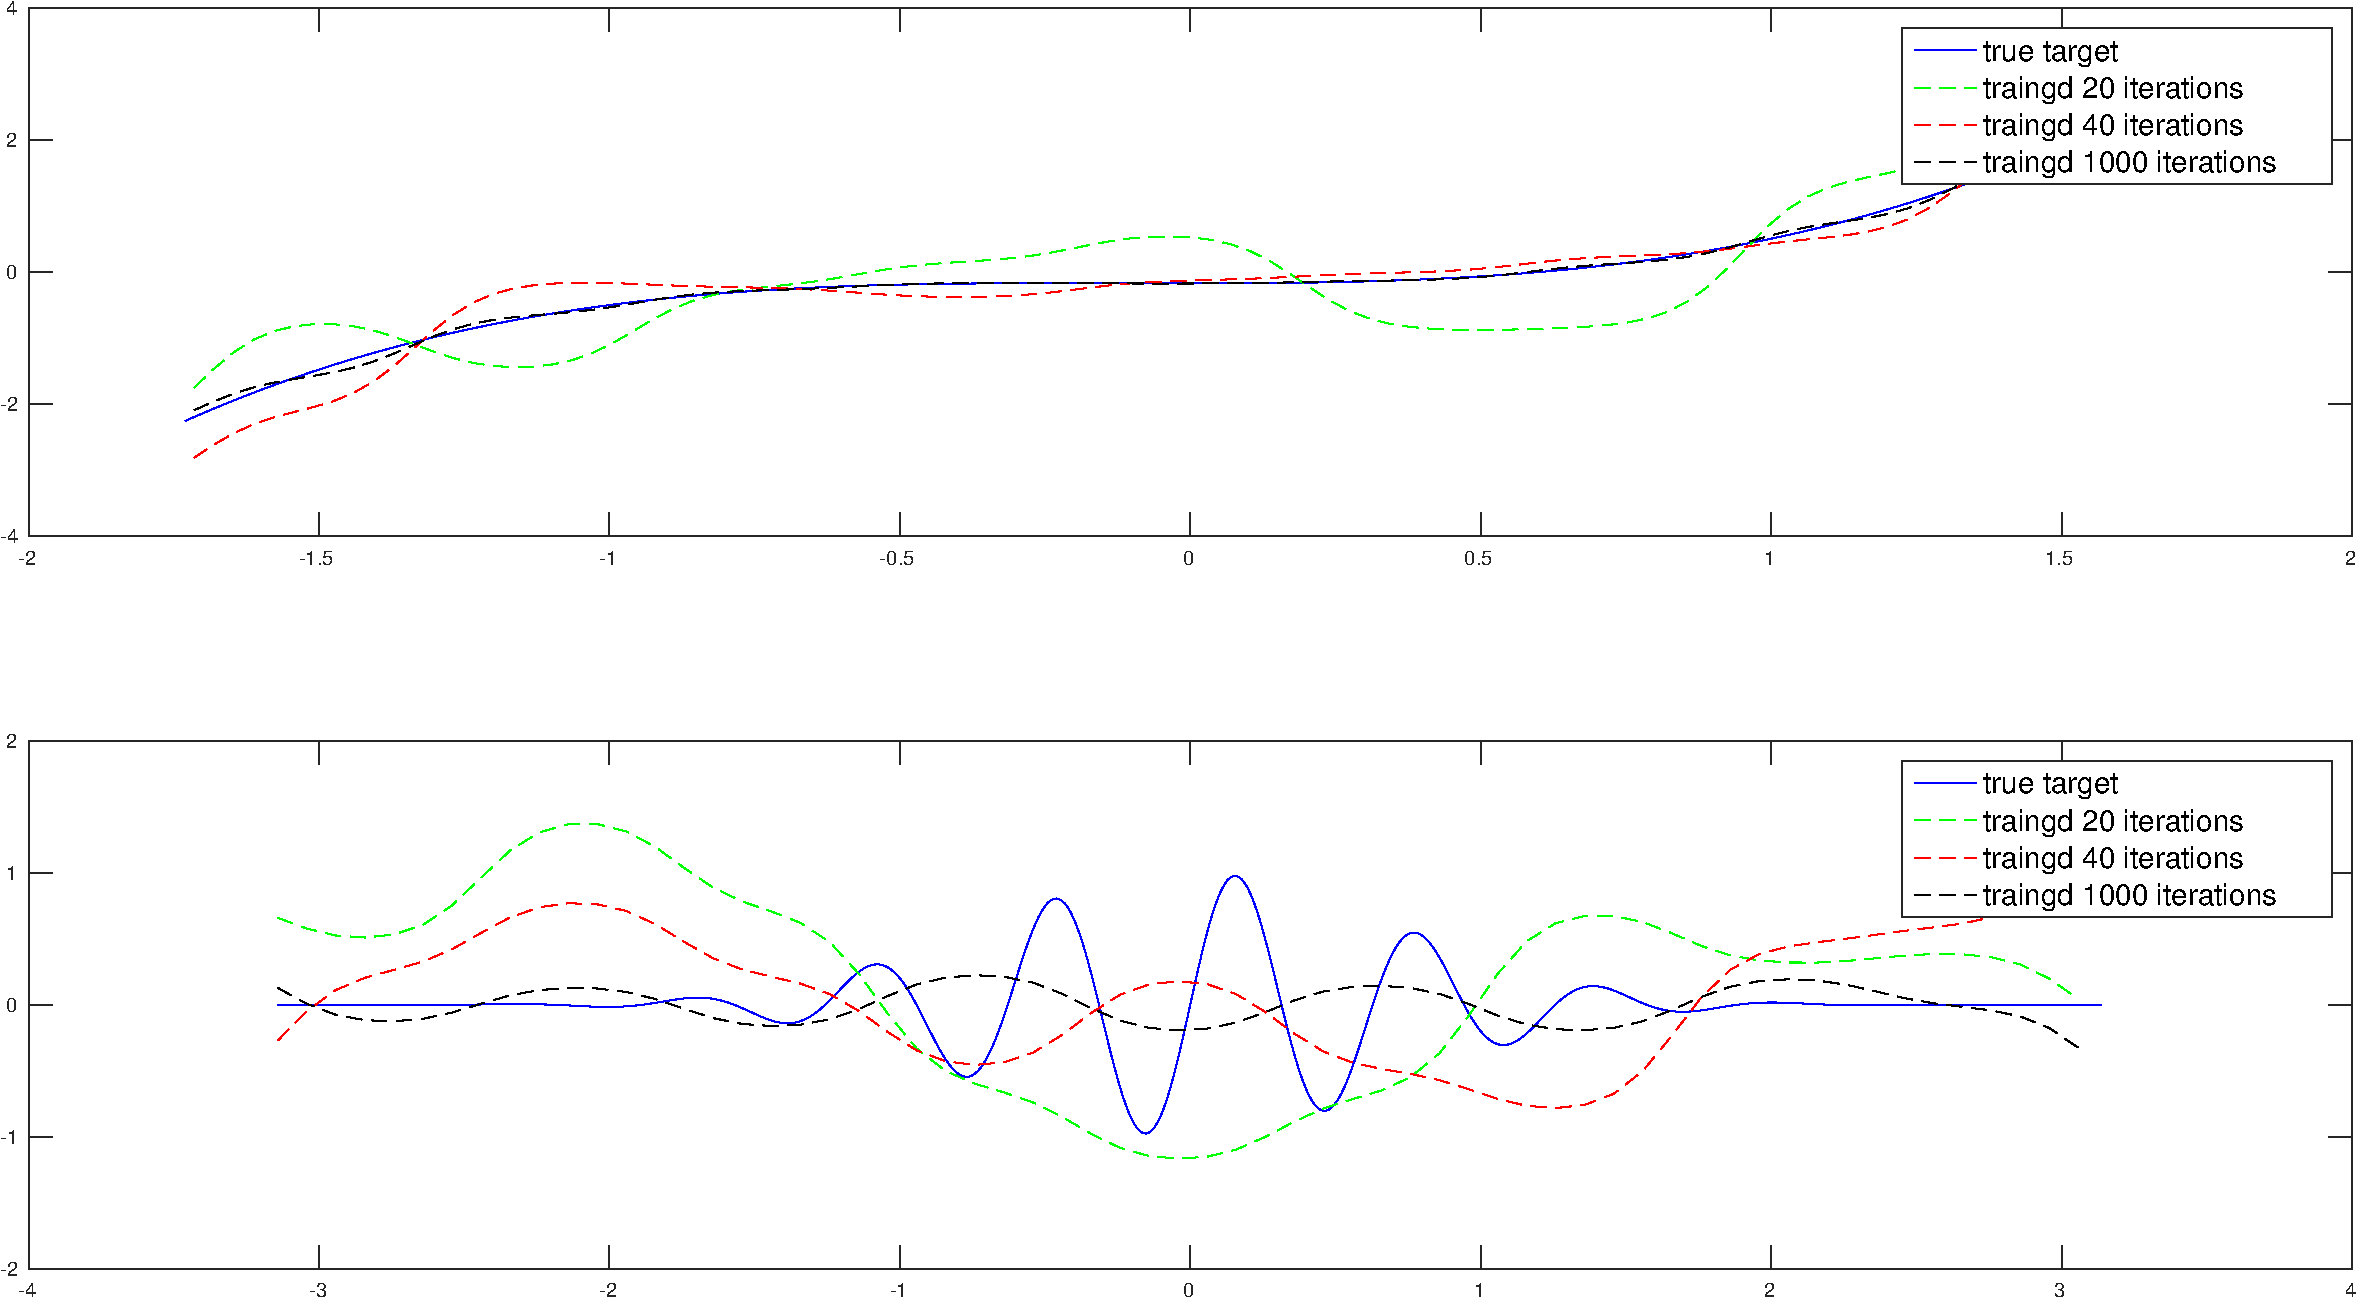
\includegraphics[scale=.43]{traingd.pdf}
  \caption{Training with gradient descent}
  \label{fig:traingd}
\end{figure}

On the other hand, other learning methods worked really well with the
2 functions. The results in terms of fitting and performance are
illustrated in \ref{fig:trainll}

\begin{figure}[H]
  % \centering
  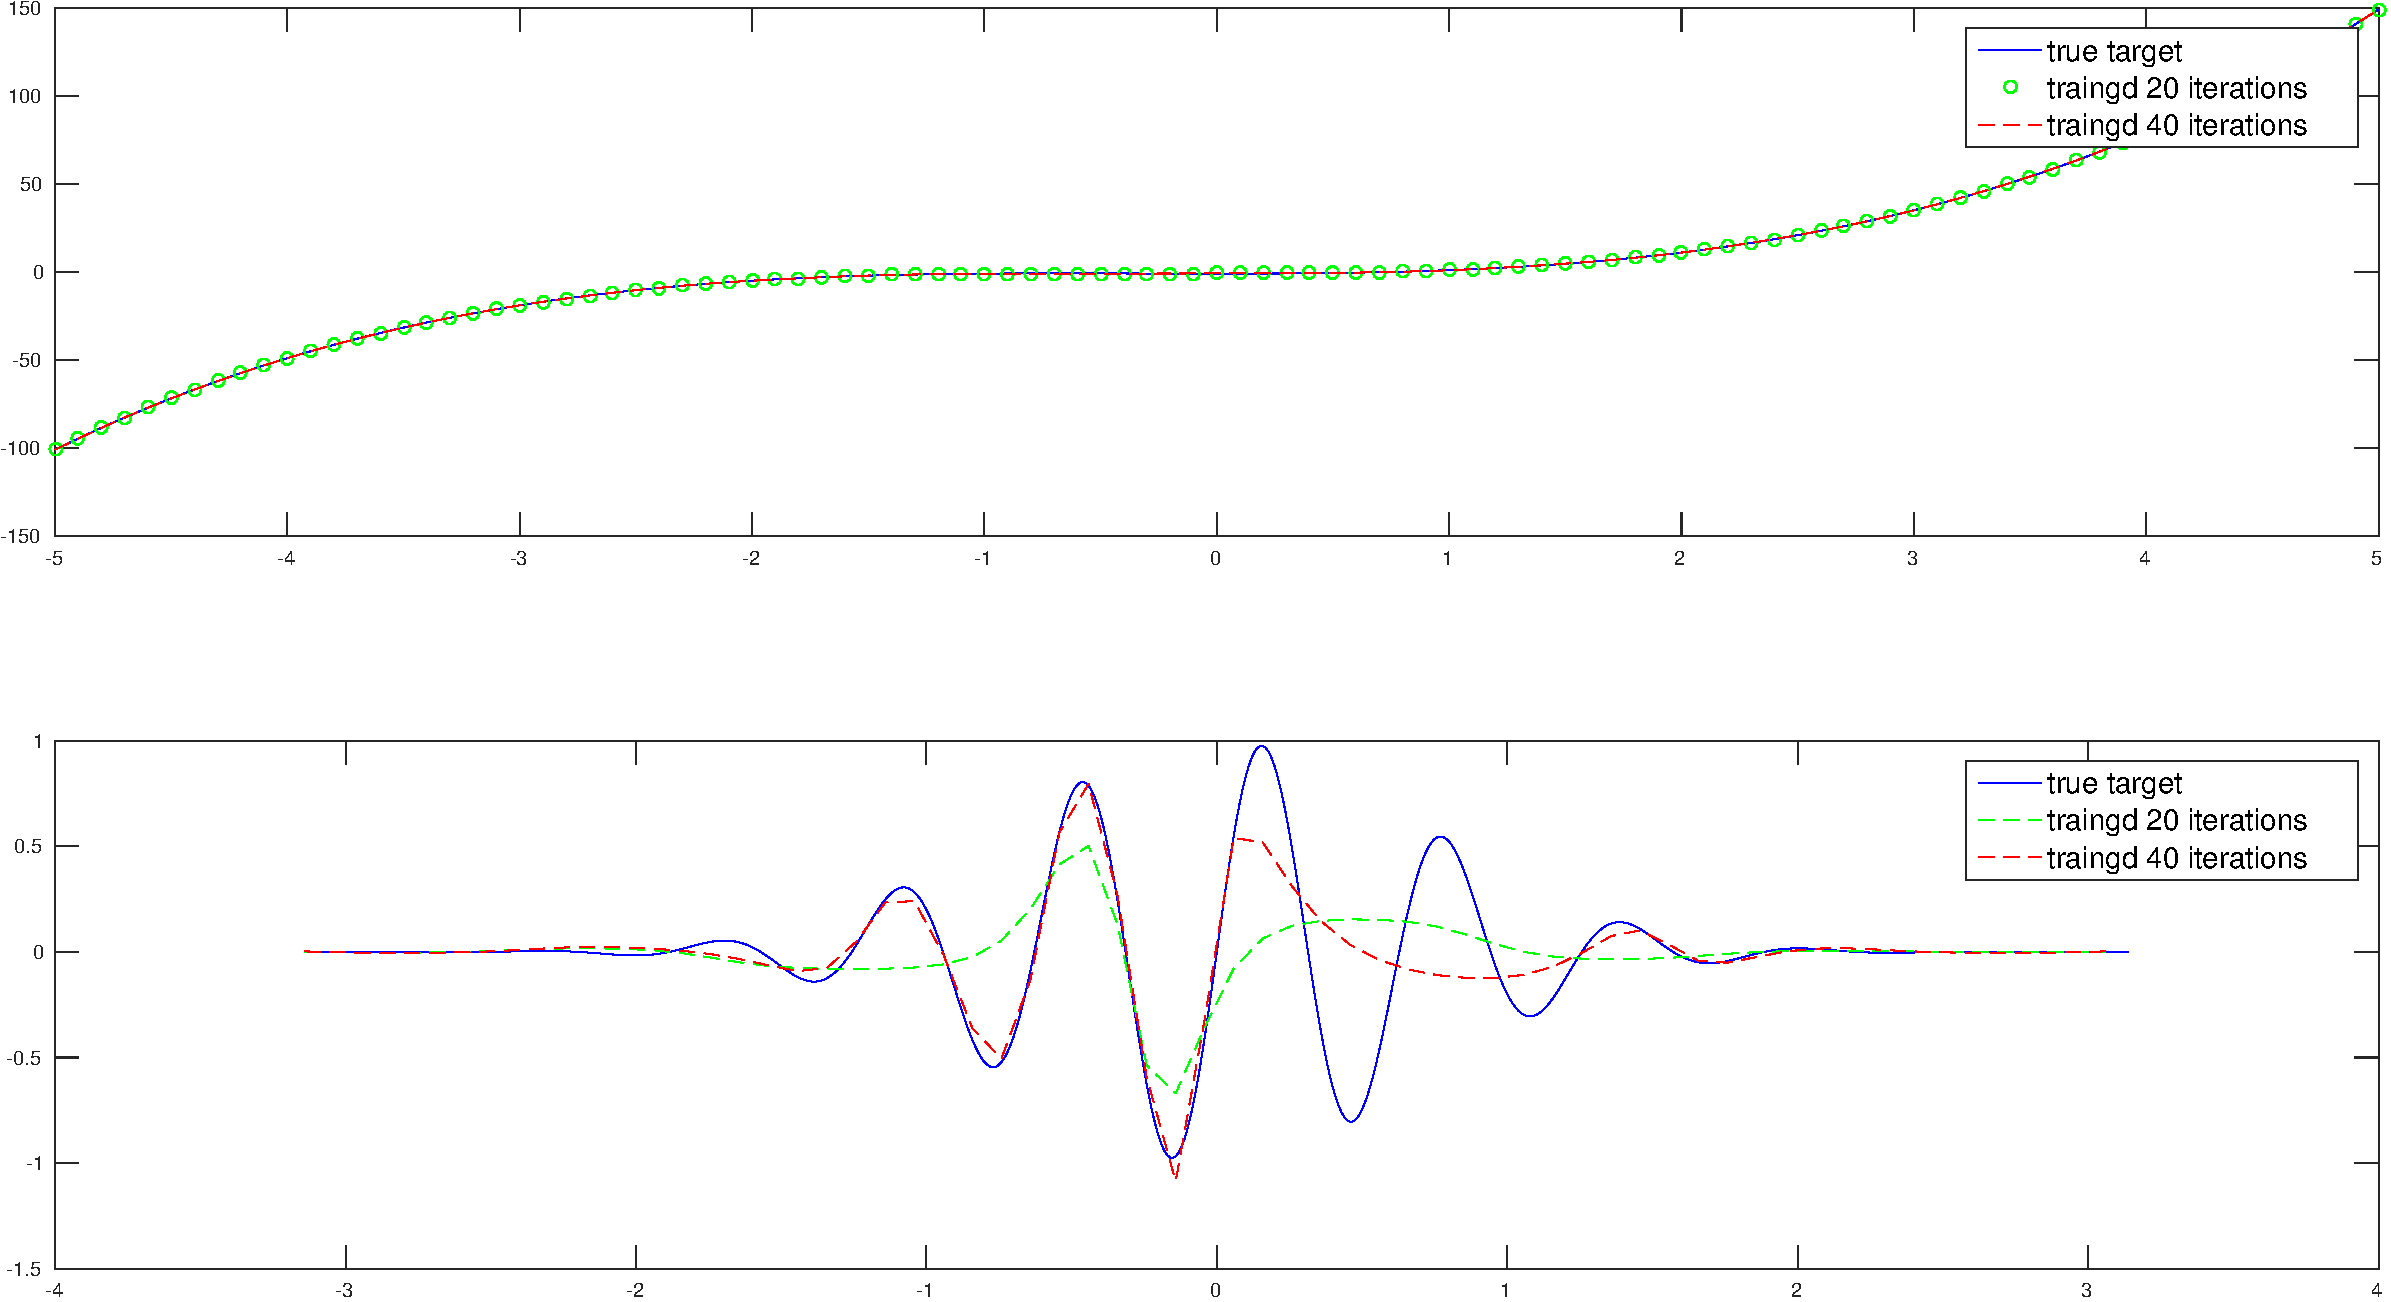
\includegraphics[scale=.43]{trainlm.pdf}
  \caption{Training with gradient descent}
  \label{fig:trainll}
\end{figure}

\section{Noisy learning}


\bibliographystyle{ieeetr} 
\bibliography{bib-db}

\end{document}
